\chapter{Introduction}\label{ch:introduction}
\section{Context}
The Standard Model of particle physics, which describes the fundamental constituents of matter and their interactions, represents an unambiguous triumph of the scientific method. Its predictions have been verified to extraordinary precision. Its last missing piece, the Higgs boson, was discovered in 2012 \cite{Aad:2012tfa,Chatrchyan:2012xdj}, fifty years after it was predicted. This resulted in a Nobel prize for Francois Englert and Peter Higgs, and in much jubilation among the particle physics community. 

\begin{marginfigure}[2.5cm]
  \centering
  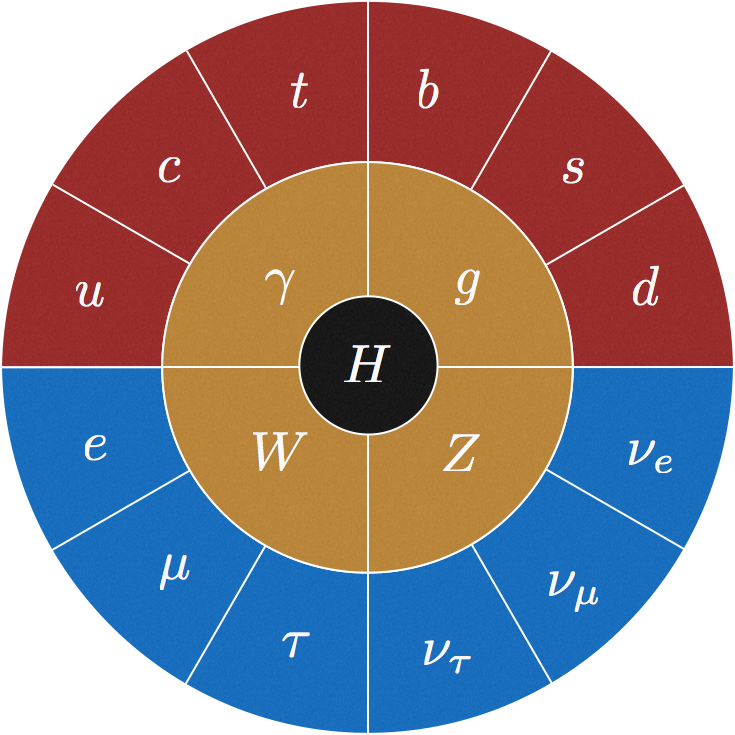
\includegraphics[width=0.8\textwidth]{images/SM-wheel.png}
  \caption{Graphical representation of the particle content of the standard model Source: the movie \emph{Particle Fever} (2013).}
\end{marginfigure}

However, many questions still remain unanswered by the standard model. For example, a very basic level, the standard model does not explain why neutrinos have masses, and does not contain a viable dark matter candidate particle. On a more abstract level, the squared mass of the Higgs boson in the standard model is not protected from large radiative corrections, and seems unnaturally finely tuned - this is termed the \emph{hierarchy problem}, and we will return to it in \autoref{ch:supersymmetry}. And perhaps the greatest challenge is that of reconciling the standard model with the theory of general relativity. In fact, it is widely believed that the Standard Model is only a low-energy effective approximation to an underlying theory that is valid at higher energy scales.

To answer these questions, we must go beyond the Standard Model with new theories. These new theories often predict new fundamental particles and forces. Currently, our best tools to study these new particles are particle colliders, like the Large Hadron Collider (LHC), which lies on the border between Switzerland and France (\autoref{fig:LHC_schematic}).

\begin{figure}
  \centering
  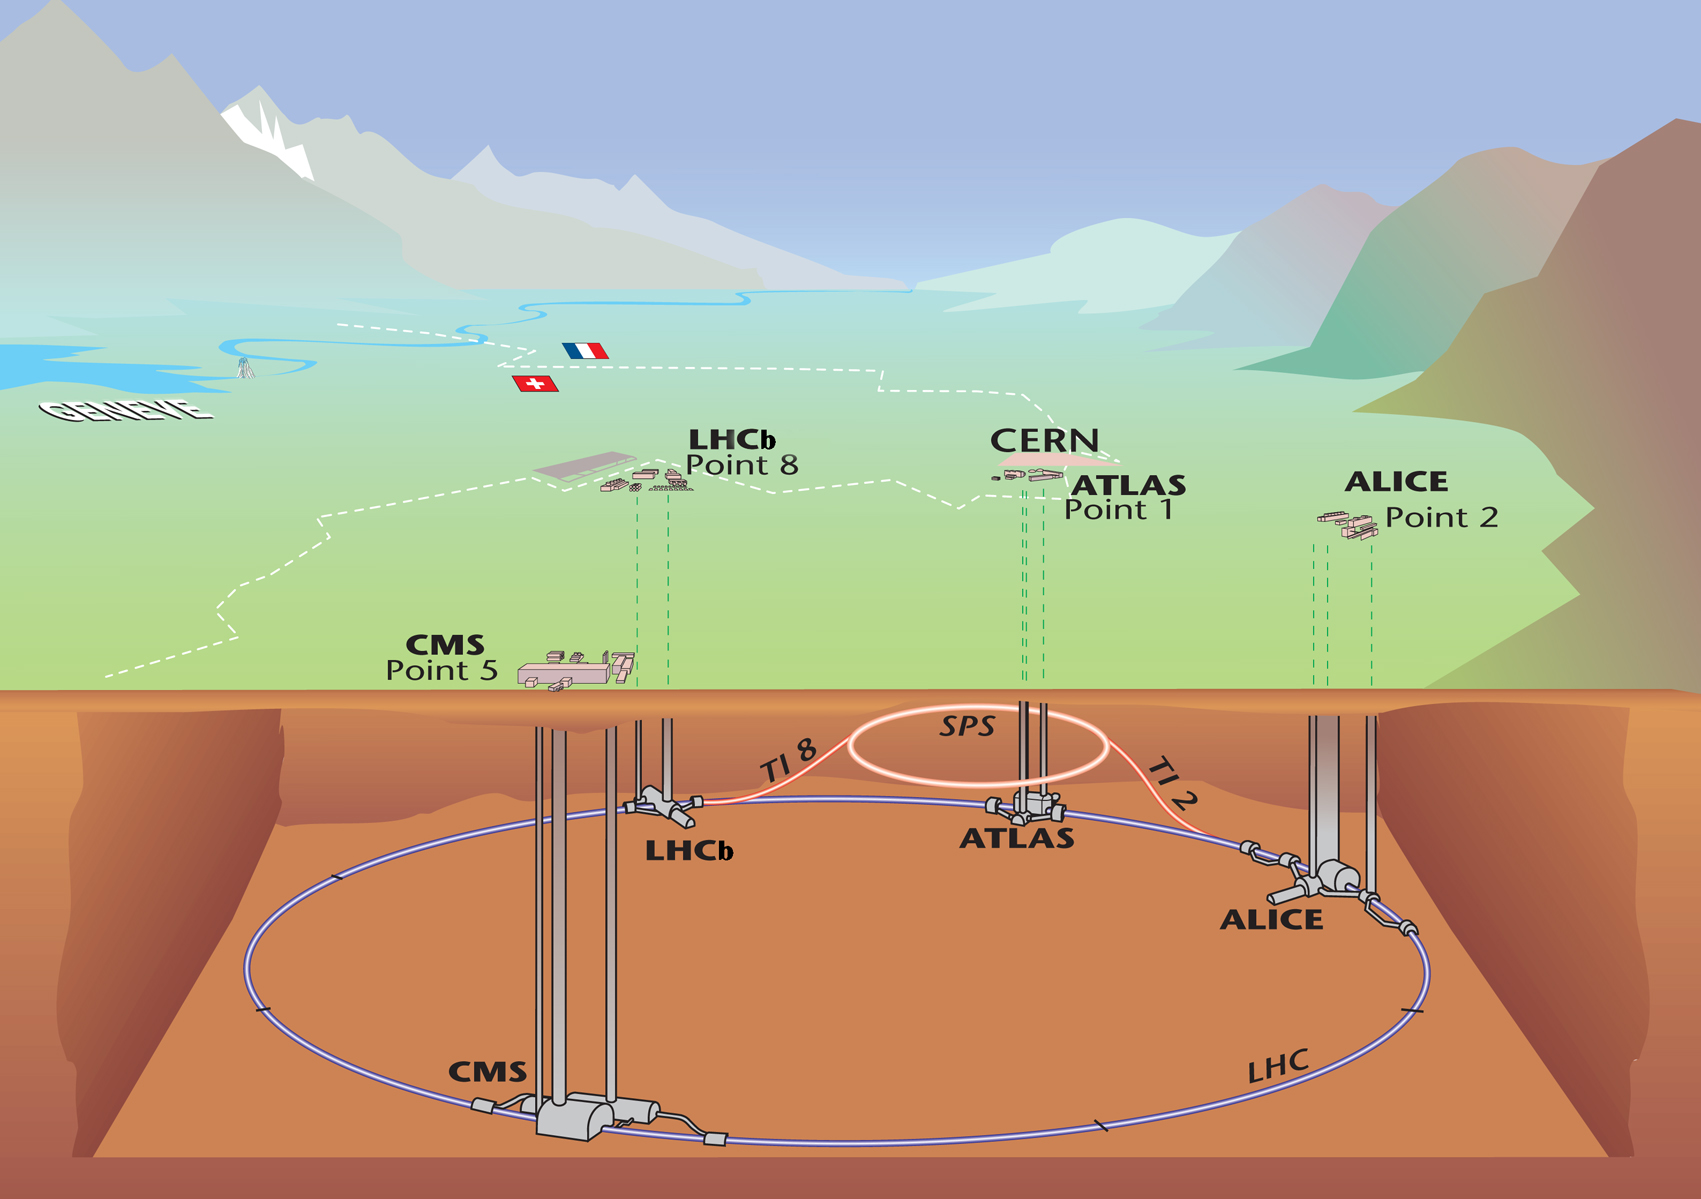
\includegraphics[width=0.9\textwidth]{images/LHC}
  \caption{Schematic diagram of the Large Hadron Collider, which lies on the border between Switzerland and France. \href{http://cds.cern.ch/journal/CERNBulletin/2008/38/News\%20Articles/1125888?ln=en}{(CERN)}}
  \label{fig:LHC_schematic}
\end{figure}

At these colliders, we collide particles at near-lightspeed, creating new particles that can be detected by extremely sophisticated detectors. One of the main challenges at particle colliders is that there are hundreds of millions of particle collisions every second, but only a small fraction of these will have signatures of new physics. In addition, there are a multitude of viable theories beyond the Standard Model, with large parameter spaces that can be tested. However, performing a full experimental analysis for even a single search channel can be very time consuming.

For this reason, existing theories must be constrained (or excluded entirely) by holding them up to the light of experimental evidence. Furthermore, we need to have a rough idea of what the most effective collider search strategies are before going ahead with a complete experimental analysis. This is where phenomenology steps in.

Phenomenology bridges the gap between theory and experiment - connecting the predictions of the former with the measurements of the latter. In this dissertation, we present three phenomenological analyses for finding physics beyond the standard model at current and future colliders. In the next section, we describe the structure of this dissertation, and contents of each chapter.

\section{Structure of the dissertation}
\subsection{\autoref{part:Theory}}
This part of the dissertation contains brief reviews of the Standard Model, Two Higgs Doublet Models, Supersymmetry, and the Minimal Supersymmetric Standard Model. The material in these chapters is adapted from a number of review articles and textbooks that are cited in the individual chapters. Some topics are elaborated on compared to the sources, while some are condensed.  While this is not new material, it is a synthesis that the author believes provides additional context and coherence to the dissertation.
\paragraph{Chapter \ref{ch:sm}} A more or less self-contained review of the Standard Model of Particle Physics, accessible to readers with a basic knowledge of quantum electrodynamics and group theory. The focus of this chapter is on motivating and developing the Glashow-Weinberg-Salam theory of electroweak interactions, since the collider analyses in this dissertation focus on electroweak decays of exotic Higgses and neutral Higgsinos. The treatment of this topic is semi-historical in nature. We also give an overview of spontaneous symmetry breaking and the Higgs mechanism, building up to electroweak symmetry breaking through examining a few simpler examples first. We briefly touch upon asymptotic freedom and QCD to introduce the concept of jets at hadron colliders. Finally, we conclude by pointing out a few of the limitations of the Standard Model, and consequently the need to formulate new theories to address them.
\paragraph{Chapter \ref{ch:2HDMs}} This chapter motivates and reviews a class of extensions to the scalar sector of the Standard Model, known as Two Higgs Doublet Models (2HDMs). The most general 2HDM scalar potential is introduced and then constrained using phenomenological motivations. The mass spectrum of the Higgs sector in such constrained models is discussed, followed by a brief listing of the Yukawa and weak interactions of these new, exotic Higgs bosons. The analyses in \autoref{ch:2HDMs} and \autoref{ch:ExoticHiggs} are designed to discover or exclude points in the parameter space of a particular kind of 2HDM, known as the Type-II 2HDM.
\paragraph{Chapter \ref{ch:supersymmetry}} The main motivations behind the development of supersymmetry are provided, followed by an introduction to the algebra of supersymmetry operators. The subsequent sections introduce the concepts of superfields and superspace and review the construction of general renormalizable supersymmetric Lagrangians. Having done this, we specialize to the Lagrangian of the Minimal Supersymmetric Standard Model, providing the superpotential, terms that softly break supersymmetry, and phenomenologically motivated simplifying assumptions. We also list the particle content of the MSSM, grouped by chiral and gauge supermultiplets. Finally, we conclude with a brief discussion of the implications of a supersymmetric spectrum with a mass hierarchy between fermionic and scalar superpartners of the SM particles. The MSSM is a special instance of a Type-II 2HDM, and the analysis in \autoref{ch:DM_100_TeV} is designed to explore the parameter space of the MSSM with a split spectrum.  
\subsection{\autoref{Part:Phenomenology}}
We provide a brief introduction to collider phenomenology and the role that machine learning can play in it. This part represents the author's own attempt at a narrative that bridges theory and experiment, as well as an attempt to cast particle physics concerns in the language of machine learning.
\paragraph{Chapter \ref{ch:ColliderPheno}} This chapter describes how to connect theoretical predictions and experimental observables. The design of a generic multipurpose detector for a hadron collider is discussed, followed by discussions of some of the kinematic variables that are relevant to our analyses in \autoref{part:Three}. We briefly comment upon a 100 TeV hadron collider as a potential successor to the LHC, and some of the physics motivations behind it. The chapter concludes with a discussion of hypothesis testing and statistical significance in particle physics.
\paragraph{Chapter \ref{ch:MachineLearning}} This chapter motivates the use of a class of techniques collectively known as statistical learning, or machine learning, in particle physics analyses. We show how the task of separating signal and background events in particle physics translates to a \emph{classification} problem in the language of machine learning. We visually illustrate the potential benefits of applying machine learning techniques to efficiently find non-linear boundaries in \emph{feature space} between signal and background events. We conclude by describing the particular machine learning classifier that we use in our analyses, the Boosted Decision Tree classifier.

\subsection{\autoref{part:Three}}
This is the heart of the dissertation, where we present three original collider analyses designed to probe Type-II 2HDMs and the MSSM at the current 14 TeV LHC and a future 100 TeV hadron collider.

\paragraph{Chapter \ref{ch:LightChargedHiggs}} 
A new type of Higgs boson, known as the \emph{charged} Higgs boson and denoted by $H^\pm$, arises naturally in the spectrum of 2HDMs. Finding one of these would be an unmistakable sign of new physics beyond the Standard Model. The mass of this particle, $m_{H^\pm}$ is a free parameter in the theory. Searches for this particle can be divided into two broad categories - the first involving charged Higgs bosons lighter than the top quark, and the other dealing with charged Higgses heavier than the top quark. In this chapter, we examine the first scenario, with charged Higgses coming from the decay of top quarks that are either produced singly or in pairs. While experimental results from CMS and ATLAS  have placed a lower limit of 160 GeV for the mass of the charged Higgs boson in the context of the MSSM, these limits have been placed assuming that the charged Higgs decays solely via `standard' channels, i.e. into SM particles. However, theories that predict charged Higgs typically predict other BSM particles as well, which can potentially be lighter than the charged Higgs, thus openining up new, `exotic' decay channels for it. For certain regions of parameter space (namely regions with low values of the parameter $\tan\beta$), the rate of these exotic decays is much larger than the rate of the decays to SM particles, thus significantly weakening the limits set by the LHC. For a complete picture, we must take into account not only the standard decay channels, but the exotic ones as well. In this chapter, we investigate one of these decay channels, that is, the weak decay of a charged Higgs to a lighter Higgs boson - either the pseudoscalar \emph{A} or the CP-even scalar \emph{H} - with a mass of 70 GeV, and a W boson. 
We first perform a \emph{model-independent} analysis. That is, \emph{assuming} that $H^\pm$ decays exclusively to $AW^\pm/HW^\pm$, and assuming that \emph{A/H} decays to a pair of tau leptons 8.6\% of the time, we set out to find the minimum rate of the signal process required for this analysis to discover it with a significance of $5\sigma$, or exclude it with a significance of $1.96\sigma$. This rate corresponds to the strength of the signal - the weaker the signal that can be probed by the analysis, the more powerful it is. The limit on the signal strength can be translated into a limit on the branching ratio (BR) of the process $t\rightarrow H^\pm b$. We determined that the single top and the top pair channels could potentially set upper limits of 0.2\% and 0.3\% respectively on the branching ratio BR($t\rightarrow H^\pm b$). For this analysis to discover the signal process, the branching ratio would have to be about three times higher than the aforementioned upper limits. These results can be translated into contours in the two-dimensional $m_{H^\pm}-\tan\beta$ plane in the parameter space of a Type-II 2HDM that delineate regions that can be either discovered or excluded with this analysis. We determined that this analysis would be able to discover points with $m_{H^\pm}$ between 155 and 165 GeV for $\tan\beta > 17$, and the entire mass range for $\tan\beta < 6$. We also found that almost the entire relevant region of the $m_{H^\pm}-\tan\beta$ plane can be excluded with this analysis, with the exception of the regions with very small mass differences between the charged Higgs and the top quark. In summary, we found that the exotic decay channel $H^\pm\rightarrow AW^\pm/HW^\pm$ probes a region of parameter space complementary to the region probed by standard decay channels (such as $H^\pm\rightarrow \tau\nu$), and thus is an important search channel to consider in the context of 2HDMs.
The results in this chapter have been published as an article in the Journal of High Energy Physics \citep{Kling2015c}. While the contents of the chapter have been edited to avoid redundancy and integrate it more tightly into the thesis, there will inevitably be a substantial overlap between chapter and the published article. The article was coauthored with Felix Kling and Shufang Su. The collider analysis for the top pair production channel, as well as the calculation of the limits  was carried out by Felix. The collider analysis for the single top production channel was carried out by the author of this dissertation.  

\paragraph{Chapter \ref{ch:DM_100_TeV}}
A 100 TeV proton-proton collider will be an extremely effective way to probe the electroweak sector of the Minimal Supersymmetric Standard Model (MSSM). In this chapter, we describe a search strategy for discovering pair-produced higgsino\footnote{Higgsinos are the fermionic counterparts of scalar Higgs fields. The title of the dissertation is thus potentially a less than rigorous interpretation of the term `Higgses' - but the alliteration was just too good to pass up.}-like neutralinos $\tilde{\chi}_{2,3}^0$ that decay to the lightest neutralino $\tilde{\chi}_1^0$ (which we assume to be an almost pure bino). We investigate the particular case in which the higgsinos decay via intermediate \emph{Z} and SM Higgs bosons \emph{h}, that in turn decay to a pair of leptons and a pair of b-quarks respectively: 
$$\tilde{\chi}^0_{2,3}\tilde{\chi}^0_{3,2}\rightarrow (Z\tilde{\chi}^0)(h\tilde{\chi}_1^0)\rightarrow bbll+\tilde{\chi}_1^0\tilde{\chi}_1^0.$$
We performed two analyses simultaneously - the first using rectangular selection cuts on physically motivated kinematic observables known as razor variables, and the second using the same high-level observables, along with a few lower-level observables as input features for a Boosted Decision Tree Classifier. The results show that the machine learning technique performs substantially better than the regular rectangular selection cuts. With the machine learning analysis, we would be able to discover higgsinos up to a mass of 1.3 TeV, and exclude them to up to a mass of 1.8 TeV. Correspondingly, we can discover binos up to 900 GeV, and exclude them up to 1.3 TeV. The research for this chapter was carried out by the author under the guidance of Shufang Su, and forms the basis of a completed manuscript that will soon be submitted for publication in the Journal of High Energy physics. 

\paragraph{Chapter \ref{ch:ExoticHiggs}}
While the project that \autoref{ch:LightChargedHiggs} is based on dealt with the implications of additional, exotic decay channels opening up for charged Higgs bosons arising from extended scalar sectors at the LHC, the project that this chapter is based on is much more ambitious in scope, aiming for nothing less than a complete prospectus of exotic Higgs decay channels in 2HDMs with large mass hierarchies. The authors of \citep{Kling2016} have presented a collection of promising 2HDM benchmark planes for investigation at the LHC that take into account theoretical and experimental constraints, and highlight the complementarity between the different search channels. The end goal of this project is to perform detailed collider analyses to determine exclusion and discovery bounds for both the original benchmark planes at the 14 TeV LHC, as well as extended benchmark planes at a 100 TeV collider that reflect the higher obtainable mass reach. In this chapter, we present preliminary results based on collider analyses carried out for one of the benchmark planes, corresponding to the mass hierarchy $m_H < m_A = m_{H^\pm}$. The exotic decay channels considered are $A\rightarrow HZ$ and $H^\pm\rightarrow HW^\pm$. As already shown in \autoref{ch:DM_100_TeV}, machine learning techniques represent a substantial improvement over rectangular selection cuts. Taking this and the extremely large number of benchmark points we need to scan across into account, the analyses in this chapter are based solely on Boosted Decision Tree classifiers. Using this technique, we are able to exclude the following regions in the benchmark plane: (insert excluded ranges here)

This work is being done in collaboration with Felix Kling, Huayang Song, Honglei Li, and Shufang Su. The results for the $A\rightarrow HZ$ channels have been obtained by Huayang and Honglei by using and extending analysis code originally written by Felix, while the results for the $H^\pm\rightarrow HW^\pm$ decay channel have been obtained by the author using code that builds upon that of \autoref{ch:DM_100_TeV}. The Monte Carlo event samples for all the channels at 100 TeV were generated by the author on the University of Arizona computing cluster. 
%Generating these samples for hundreds of signal benchmark points and backgrounds with extremely large cross sections is not a trivial task (and even less so at 100 TeV), and requires careful management of computational resources. During the course of performing the research that comprises this dissertation, the author has developed a Python-based framework, \texttt{clusterpheno}, for event generation and analysis on a cluster. An advantage of using this over the CMS gridpack method is that the entire pipeline of MadGraph-Pythia-Delphes is integrated

In some ways, the three analyses presented in this dissertation can be viewed as a progression on two fronts. On the one hand, they involve increasingly high collider energies, going from 14 TeV to 100 TeV. On the other, they involve an increasing use of machine learning techniques. The first analysis solely uses rectangular selection cuts, the second qualitatively compares rectangular cut and machine learning strategies, and the third uses machine learning exclusively. The author believes that it is likely that this trend will be reflected in experimental particle physics research in the future, as we attempt to grapple with increasingly difficult questions at the frontier of the field

\paragraph{Open Science} The author strongly believes in the value of reproducible research and open science. In this spirit, the source code for the dissertation document has been made freely available online at

\url{https://github.com/adarshp/dissertation}.

\noindent The code for the analysis in \autoref{ch:DM_100_TeV} can be found at

\url{https://github.com/adarshp/Dark-Matter-at-100-TeV}

\noindent while the code for the analysis of the $H^\pm\rightarrow HW^\pm$ decay channel in \autoref{ch:ExoticHiggs} can be found at

\url{https://github.com/adarshp/ExoticHiggs}.

\noindent In addition, the code for both of these analyses utilizes a Python-based software framework, \texttt{clusterpheno}, written by the author during the course of his graduate work, for the purpose of performing large-scale event generation and analysis on the University of Arizona cluster. The source code for this framework can be found online at 

\url{https://github.com/adarshp/clusterpheno}.
